\documentclass{article}

\usepackage{fancyhdr}
\usepackage{extramarks}
\usepackage{amsmath}
\usepackage{amsthm}
\usepackage{amsfonts}
\usepackage{tikz,pgfplots}
\usepackage[plain]{algorithm}
\usepackage{algpseudocode}
\usepackage[]{mcode}
\usepackage{graphicx}
\usepackage{epstopdf}
\usepackage{siunitx}

\usetikzlibrary{automata,positioning}

%
% Basic Document Settings
%

\topmargin=-0.45in
\evensidemargin=0in
\oddsidemargin=0in
\textwidth=6.5in
\textheight=9.0in
\headsep=0.25in

\linespread{1.1}

\pagestyle{fancy}
\lhead{\hmwkAuthorName}
\chead{\hmwkClass\ (\hmwkClassInstructor\ \hmwkClassTime): \hmwkTitle}
\rhead{\firstxmark}
\lfoot{\lastxmark}
\cfoot{\thepage}

\renewcommand\headrulewidth{0.4pt}
\renewcommand\footrulewidth{0.4pt}

\setlength\parindent{0pt}

%
% Create Problem Sections
%

\newcommand{\enterProblemHeader}[1]{
    \nobreak\extramarks{}{Problem \arabic{#1} continued on next page\ldots}\nobreak{}
    \nobreak\extramarks{Problem \arabic{#1} (continued)}{Problem \arabic{#1} continued on next page\ldots}\nobreak{}
}

\newcommand{\exitProblemHeader}[1]{
    \nobreak\extramarks{Problem \arabic{#1} (continued)}{Problem \arabic{#1} continued on next page\ldots}\nobreak{}
    \stepcounter{#1}
    \nobreak\extramarks{Problem \arabic{#1}}{}\nobreak{}
}

\setcounter{secnumdepth}{0}
\newcounter{partCounter}
\newcounter{homeworkProblemCounter}
\setcounter{homeworkProblemCounter}{1}
\nobreak\extramarks{Problem \arabic{homeworkProblemCounter}}{}\nobreak{}

%
% Homework Problem Environment
%
% This environment takes an optional argument. When given, it will adjust the
% problem counter. This is useful for when the problems given for your
% assignment aren't sequential. See the last 3 problems of this template for an
% example.
%
\newenvironment{homeworkProblem}[1][-1]{
    \ifnum#1>0
        \setcounter{homeworkProblemCounter}{#1}
    \fi
    \section{Problem \arabic{homeworkProblemCounter}}
    \setcounter{partCounter}{1}
    \enterProblemHeader{homeworkProblemCounter}
}{
    \exitProblemHeader{homeworkProblemCounter}
}

%
% Homework Details
%   - Title
%   - Due date
%   - Class
%   - Section/Time
%   - Instructor
%   - Author
%

\newcommand{\hmwkTitle}{Tutorial\ 3}
\newcommand{\hmwkDueDate}{March 31, 2017}
\newcommand{\hmwkClass}{Digital Signal Processing}
\newcommand{\hmwkClassTime}{}
\newcommand{\hmwkClassInstructor}{Friso DeBoer}
\newcommand{\hmwkAuthorName}{S.Reynolds (262538)}

%
% Title Page
%

\title{
    \vspace{2in}
    \textmd{\textbf{\hmwkClass:\ \hmwkTitle}}\\
    \normalsize\vspace{0.1in}\small{Due\ on\ \hmwkDueDate\ at 3:00pm}\\
    \vspace{0.1in}\large{\textit{\hmwkClassInstructor\ \hmwkClassTime}}
    \vspace{3in}
}

\author{\textbf{\hmwkAuthorName}}
\date{}

\renewcommand{\part}[1]{\textbf{\large Part \Alph{partCounter}}\stepcounter{partCounter}\\}

%
% Various Helper Commands
%

% Useful for algorithms
\newcommand{\alg}[1]{\textsc{\bfseries \footnotesize #1}}

% For derivatives
\newcommand{\deriv}[1]{\frac{\mathrm{d}}{\mathrm{d}x} (#1)}

% For partial derivatives
\newcommand{\pderiv}[2]{\frac{\partial}{\partial #1} (#2)}

% Integral dx
\newcommand{\dx}{\mathrm{d}x}

% Alias for the Solution section header
\newcommand{\solution}{\textbf{\large Solution}}

% Probability commands: Expectation, Variance, Covariance, Bias
\newcommand{\E}{\mathrm{E}}
\newcommand{\Var}{\mathrm{Var}}
\newcommand{\Cov}{\mathrm{Cov}}
\newcommand{\Bias}{\mathrm{Bias}}

\begin{document}

\maketitle

\pagebreak


\section{2.1 MATLAB Synthesis of Chirp Signal}
\subsection{Part A}
This section requires a chirp signal to be synthesised. The code used to answer this question is as follows:

\begin{lstlisting}
	%%%%%%%%%%%% 2.1 MATLAB Synthesis of Chirp Signals %%%%%%%%%%%%%%%
	
	% Clear the workspace and any stored variables
	clear; clc;
	
	fsamp = 8000;
	dt = 1/fsamp;
	dur = 1.8;
	tt = 0:dt:dur;
	psi = 2*pi*(100 + 200*tt + 500*tt.*tt);
	xx = real(exp(j*psi));
	
	sound(xx,fsamp);
\end{lstlisting}

A chirp signal is a signal with a time varying phase. Generally, this can be written as:
\begin{align}
	x(t) = A \cdot \cos(\psi(t))
\end{align}

The time varying phase is denoted as $\psi(t)$, and for a chirp signal this function is given by:
\begin{align}
	\psi(t) = 2 \pi \mu t^2 + 2 \pi f_0 t + \phi
\end{align}

The instantaneous frequency for a signal with a time varying phase is given by:
\begin{align}
	f_i(t) = \frac{1}{2 pi} \cdot \frac{d}{dt} \psi(t)
\end{align}

For a chirp signal the instantaneous frequency, $f_i(t)$, is linear - shown below:
\begin{align}
	 f_i(t)= 2 \mu t + f_0
\end{align}

Since the instantaneous is monotonic and linearly increasing, we note that the minimum frequency will occur when $t = 0$ and the maximum frequency will occur when $t = t_{max}$. We first need to find the parameters $\mu$ and $f_0$. In the script, we note that:
\begin{align}
	\psi(t) = 2 \pi \mu t^2 + 2 \pi f_0 t + \phi = 2 \pi \cdot 500 \cdot t^2 + 2 \pi \cdot 200 \cdot t + 2 \pi \cdot 100
\end{align}

Polynomial equality suggests that $\mu = 500$, and $f_0 = 200$. Hence, we can find both $f_{min}$ and $f_{max}$:
\begin{align}
	f_{min} &= 2 \mu \cdot 0 + f_0 = 200 \si{\hertz}\\
	f_{max} &= 2 \mu \cdot 0 + f_0 = 2 \cot 500 \cdot 1.8 + 200 = 2000 \si{\hertz}
\end{align}

A sketch of the instantaneous frequency versus time can be seen in Figure 1.
\begin{figure}[H]
	\centering
	\begin{tikzpicture}
	\centering
		\begin{axis}[
		    axis lines = left,
		    xlabel = $t$,
		    ylabel = {$f_i(t)$},
		    ymax = 2200
		]
		%Below the red parabola is defined
		\addplot [
		    domain=0:1.8, 
		    samples=100, 
		    color=red,
		]
		{2*500*x+200};
		 
		\end{axis}
	\end{tikzpicture}
	\caption{A plot of the linear instantaneous frequency for the chirp signal with parameters $\mu = 500 \si{\hertz}$, and $f_0 = 200 \si{\hertz}$}
\end{figure}

\subsection{Part B}

A function was implemented in MATLAB which created a chirp signal between two frequencies for some duration at a given sampling frequency. The code is as follows:
\begin{lstlisting}
	function xx = mychirp(f1,f2,dur,fsamp)
	% usage: xx = mychirp(f1,f2,dur,fsamp)
	% f1 = starting frequency
	% f2 = ending frequency
	% dur = total time duration
	% fsamp = sampling frequency (OPTIONAL: default is 8000)
	
	    if (nargin < 4) %--Allow optional input arguement
	        fsamp = 8000;
	    end
	    
	    dt = 1/fsamp;
	    tt = 0:dt:dur;
	    
	    f0 = f1;
	    mu = (f2 - f1)/(2*dur);
	    
	    psi = 2*pi*(mu*tt.^2 + f0*tt + 100);
	    
	    xx = real(exp(j*psi));
	    
	end
\end{lstlisting}

The function was executed to create a signal identical to that in part A. A spectrogram of the created waveform can be seen in Figure 2.
\begin{figure}[H]
	\centering
	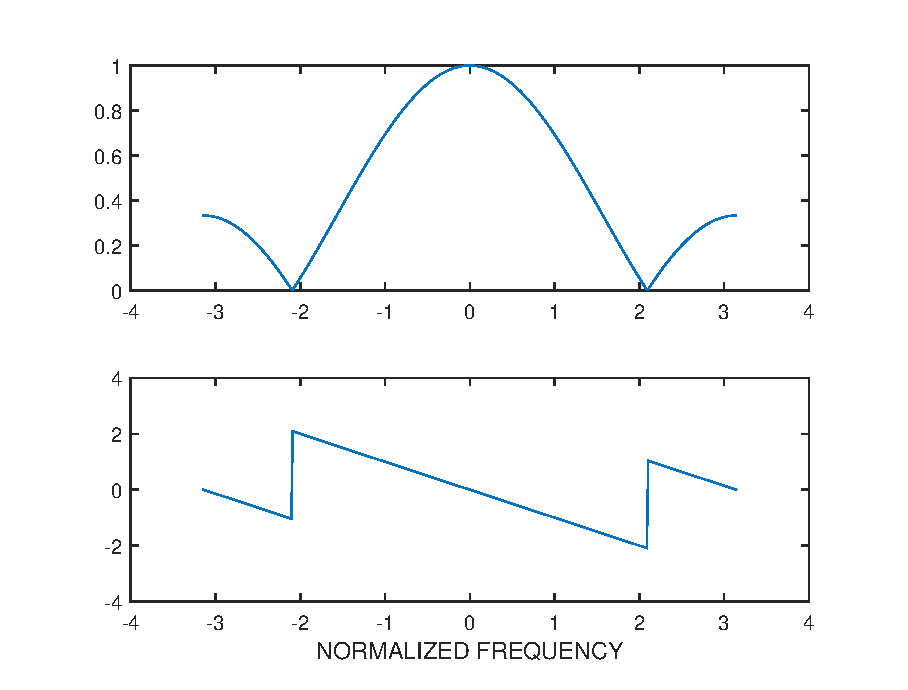
\includegraphics[scale=0.8]{fig2}
	\caption{A spectrogram of a chirp signal with starting frequency of 200 $\si{\hertz}$ and a final frequency of 2000 $\si{\hertz}$}
\end{figure}

\section{3.1 Synthesise a Chirp}
A chirp signal was synthesised between 15000$\si{\hertz}$ and 300$\si{\hertz}$. The script is shown below:
\begin{lstlisting}
	%%%%%%%%%%%%%%%%%%% 3.1 Synthesize a Chirp %%%%%%%%%%%%%%%%%%%%%%%
	
	% Clear the workspace and any stored variables
	clear; clc;
	
	% Set the duration
	dur = 3;
	
	% Set the sampling frequency
	fsamp = 8000;
	
	% Set the starting frequency and the ending frequency
	f1 = 15000;
	f2 = 300;
	
	% Create the chirp signal using mychirp
	xx = mychirp(f1,f2,dur,fsamp);
	
	% Pass the discrete time signal to the D-to-A converter
	sound(xx,fsamp)
\end{lstlisting}

The chirp sound goes up then down. The cycle repeats again - up then down. A spectrogram showing how the frequency changes with respect to time can be seen in Figure 3.

\begin{figure}[H]
	\centering
	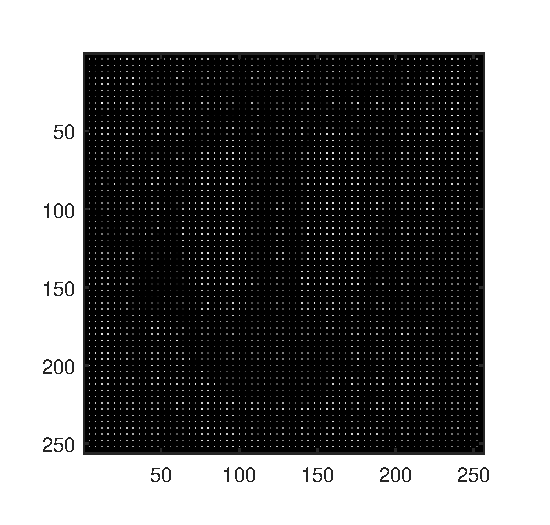
\includegraphics[scale=0.8]{fig3}
	\caption{Spectogram of a chirp signal with start frequency of 15000$\si{\hertz}$ and stop frequency of 300$\si{\hertz}$. The sampling frequency is 8000$\si{\hertz}$}
\end{figure}

The frequency rises, and then falls because the sampling rate is not high enough. Shannon's sampling theorem tells us that in order to avoid the effects of aliasing, we need to ensure that:
\begin{align}
	f_s \geq 2 \cdot f_{max}
\end{align}

Equation (3) tells us that the sampling frequency needs to be at least twice as big as the maximum frequency in the waveform. We see that at the signal starts at a frequency of 15000$\si{\hertz}$, and the sampling frequency is only 8000$\si{\hertz}$. Hence, we experience aliasing.

\section{3.2 Beat Notes}
A beat note can be thought of in two different ways: one as a modulated signal, and the second as a the sum of two distinct signals with frequencies which differ by a small amount, $f_{\Delta}$. The expression for the second way of thinking about beat notes can be seen in equation (4):
\begin{align}
	x(t) = A \cdot \cos(2 \pi (f_c - f_{\Delta})t) + B \cdot \cos(2 \pi (f_c + f_{\Delta})t)
\end{align}

A MATLAB function was implemented which created a beat note with the following script:
\begin{lstlisting}
	function [xx, tt] = beat(A, B, fc, delf, fsamp, dur)
	% BEAT compute samples of the sum of two cosine waves
	% usage:
	% [xx, tt] = beat(A, B, f, delf, fsamp, dur)
	% A = amplitude of lower frequency cosine
	% B = amplitude of higher frequency cosine
	% fc = center frequency
	% delf = frequency difference
	% fsamp = sampling rate
	% dur = total time duration in seconds
	% xx = output vector of samples
	%--OPTIONAL Output:
	% tt = time vector corresponding to xx
	    
	    % Create the time vector
	    tt = 0:(1/fsamp):dur;
	    
	    % Create the lower frequency waveform
	    xl = A*exp(j*2*pi*(fc - delf)*tt);
	    % Create the upper frequency waveform
	    xu = B*exp(j*2*pi*(fc + delf)*tt);
	    
	    % Create the beat signal
	    xx = real(xl + xu);
	end
\end{lstlisting}

The function was tested using a GUI provided by the tutorial, accessed with the command \verb|beatcon|. The beat wave form for a signal with $A = 10$, $B = 10$, $f_c = 1000$, $f_{\Delta} = 10$, $f_s = 8000$, and a duration of 1 second is shown in Figure 4. The period of the envelope can be clearly seen from the graph and is equal to 0.05 seconds.

\begin{figure}
	\centering
	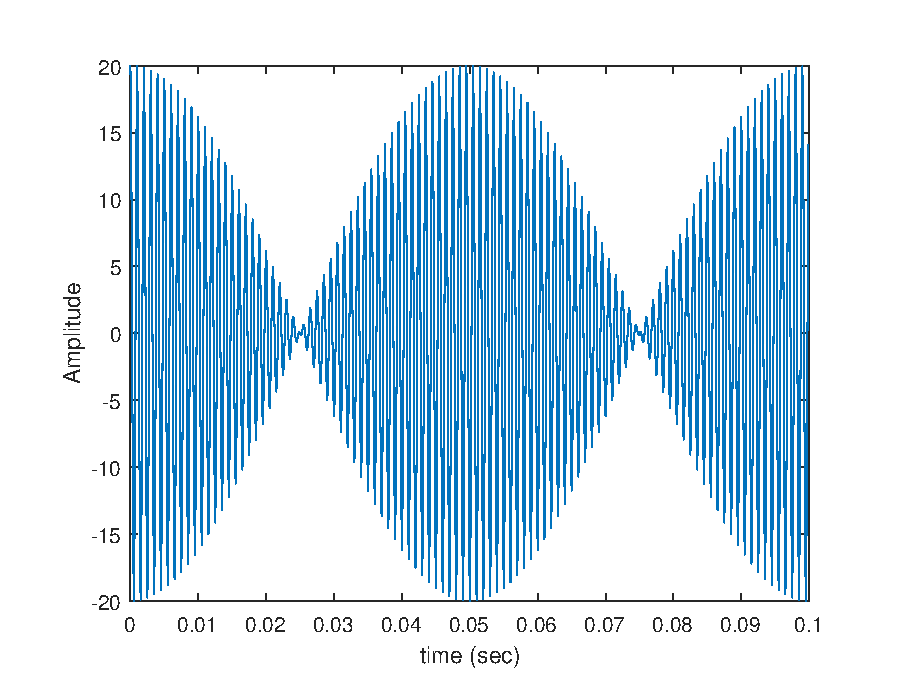
\includegraphics[scale=0.8]{fig4.eps}
	\caption{A plot of the beat waveform with parameters as described above.}
\end{figure}

\section{3.3 More on Spectrograms}
Another beat waveform was created, using the following code:
\begin{lstlisting}
	%%%%%%%%%%%%%%%%%% 3.3 More on Spectrograms %%%%%%%%%%%%%%%%%%%%%%%
	
	% Clear the workspace and clear stored variables
	clear; clc;
	
	% Specify parameters for signal generation
	delf = 32;
	fsamp = 8000;
	dur = 0.26;
	f0 = 2000;
	A = 1;
	B = 1;
	
	% Generate signal
	xx = beat(A,B,f0,delf,fsamp,dur);
	
	plot(xx)
\end{lstlisting}

Two spectrograms were plotted, and can be seen in Figures 5 and 6.

\begin{figure}[H]
	\centering
	\begin{minipage}{5cm}		
		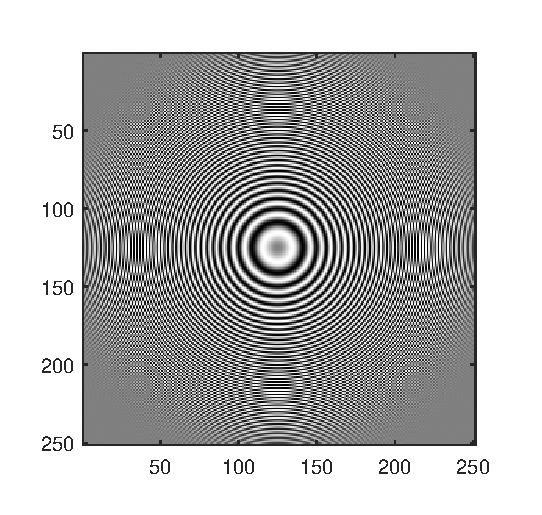
\includegraphics[scale=0.4]{fig5}
		\caption{A spectrogram of the beat signal created above using 2048 as input.}
	\end{minipage}
	\hspace{2cm}
	\begin{minipage}{5cm}
		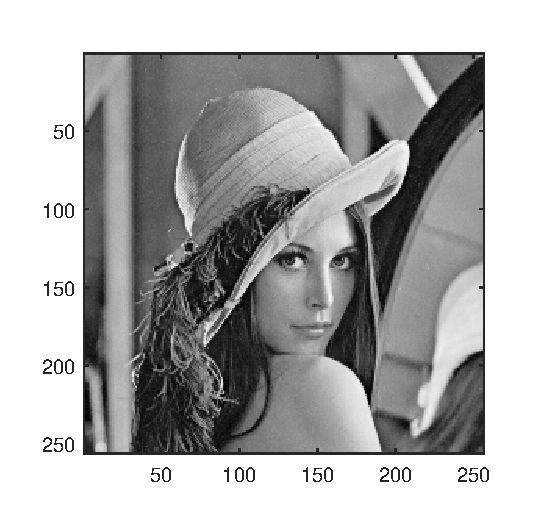
\includegraphics[scale=0.4]{fig6}
		\caption{A spectrogram of the beat signal created above using 16 as input.}
	\end{minipage}
\end{figure}

\section{4.1 Generating the Bell Envelopes}

To create a signal that sounds more like an instrument the time varying phase, $\psi(t)$, is implemented as:
\begin{align}
	\psi(t) = 2 \pi \cdot f_c \cdot t + I(t) \cdot \cos(2 \pi \cdot f_m \cdot t + \phi_m) + \phi_c
\end{align}

The composed signal is given by:
\begin{align}
	x(t) = A(t) \cdot \cos(\psi(t))
\end{align}

We note that there are two envelopes that we need to consider: $A(t)$ and $I(t)$. A decaying exponential envelope was implemented in a MATLAB function to create these envelopes:
\begin{lstlisting}
	function yy = bellenv(tau, dur, fsamp)
	% BELLENV produces envelope function for bell sounds
	% usage: yy = bellenv(tau, dur, fsamp)
	% tau = time constant
	% dur = duration of the envelope
	% fsamp = sampling frequency
	% returns:
	% yy = decaying exponential envelope
	    tt = 0:(1/fsamp):dur;
	    yy = exp(-tt./tau);
	end
\end{lstlisting}

\section{4.2 Parameters for the Bell}
A function which creates the discrete time bell signal is as follows:
\begin{lstlisting}
	function xx = bell(ff, Io, tau, dur, fsamp)
	% BELL produces a bell sound
	% usage: xx = bell(ff, Io, tau, dur, fsamp)
	% ff = frequency vector (containing fc and fm)
	% Io = scale factor for modulation index
	% tau = decay parameter for A(t) and I(t)
	% dur = duration (in sec.) of the output signal
	% fsamp = sampling rate
	    
	    % Create the time vector
	    tt = 0:(1/fsamp):dur;
	    
	    % Specify the parameters to be used
	    A = 1; % amplitude
	    phm = -pi/2; % phase constant
	    phc = -pi/2; % phase constant
	    fc = ff(1);
	    fm = ff(2);
	    
	    % Create the exponential decay envelope
	    envel = bellenv(tau, dur, fsamp);
	    
	    % Create the envelope functions A(t) and I(t)
	    At = A*envel;
	    It = Io*envel;
	    
	    % Create bell signal
	    arg = 2*pi*fc*tt + It.*real(exp(j*(2*pi*fm*tt + phm))) + phc;
	    xx = At.*real(exp(j*arg));
	end
\end{lstlisting}

\section{4.3 The Bell Sound}
The Bell function, which relies on the Bell Envelope function, was tested on a series of cases using the following script:
\begin{lstlisting}
	%%%%%%%%%%%%%%%%%% 4.3 The Bell Sound %%%%%%%%%%%%%%%%%%%%%%%%
	
	% Clear the workspace and any stored variables
	clear; clc;
	
	% Play a bell sounds
	fc = [110 220 110 110 250 250];
	fm = [220 440 220 220 350 350];
	Io = [10 5 10 10 5 3];
	tau = [2 2 12 0.3 2 1];
	dur = [6 6 3 3 5 5];
	fsamp = 11025;
	
	for i = 1:length(fc)
	    ff = [fc(i) fm(i)];
	    xx = bell(ff, Io(i), tau(i), dur(i), fsamp);
	    sound(xx,fsamp)
	    pause(dur(i)+1)
	end
\end{lstlisting}
A time series plot was created for each of the configuration of parameters a sound was played for - the time series plots can be seen in Figures 7 through 12.
\begin{figure}[H]
	\centering
	\begin{minipage}{0.3\linewidth}
		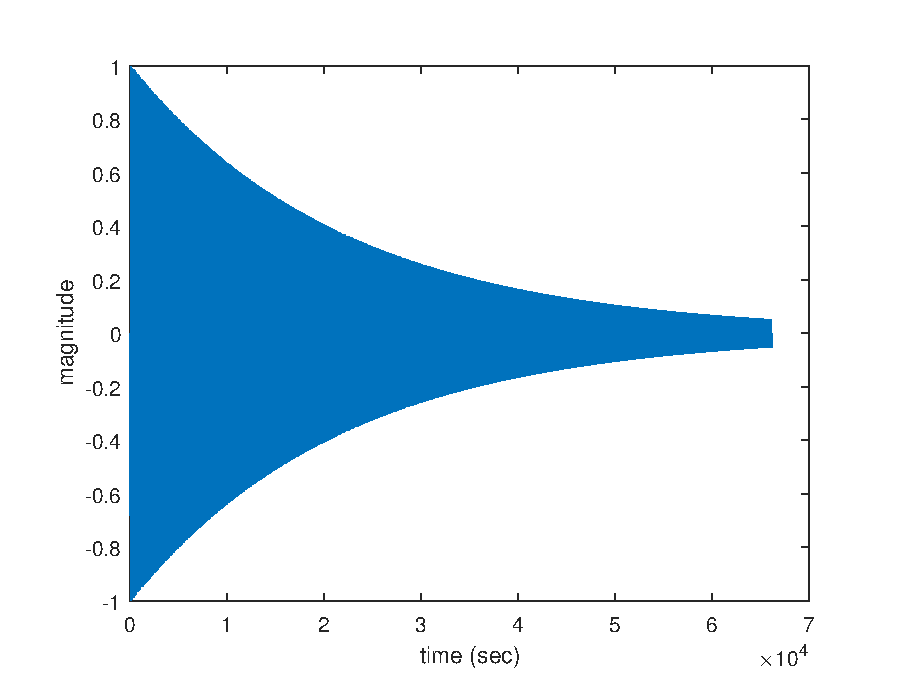
\includegraphics[scale=0.3]{time1}
		\caption{Time series plot of bell with the parameters $f_c = 110$, $f_m = 220$, $I_0 = 10$, $\tau = 2$, $T_{dur} = 6$, $f_s = 11025$}
	\end{minipage}
	\hspace{4cm}
	\begin{minipage}{0.3\linewidth}
		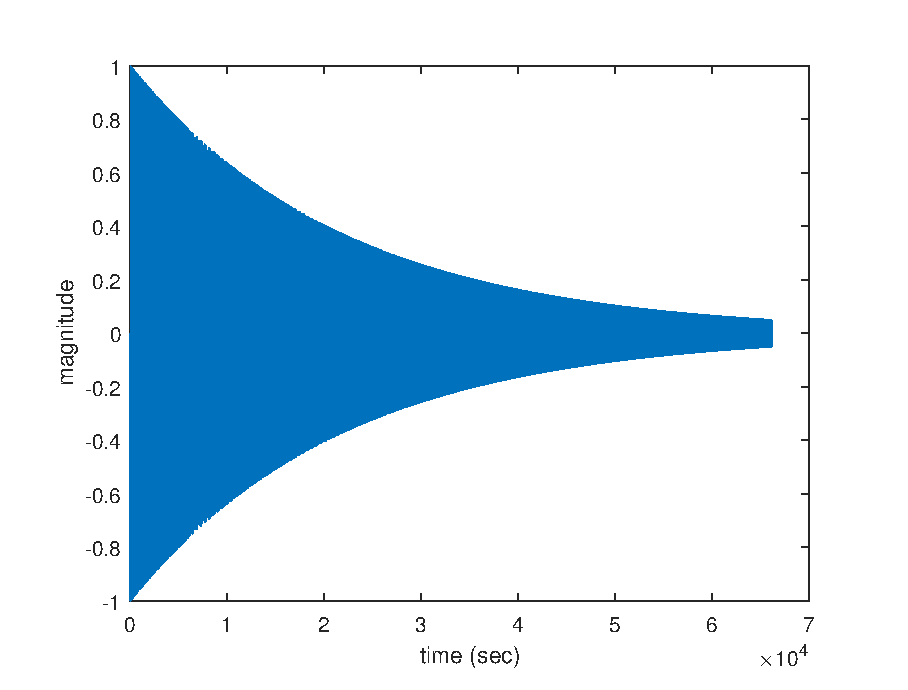
\includegraphics[scale=0.3]{time2}
		\caption{Time series plot of bell with the parameters $f_c = 220$, $f_m = 440$, $I_0 = 5$, $\tau = 2$, $T_{dur} = 6$, $f_s = 11025$}
	\end{minipage}
\end{figure}
\begin{figure}[H]
	\centering
	\begin{minipage}{0.3\linewidth}
		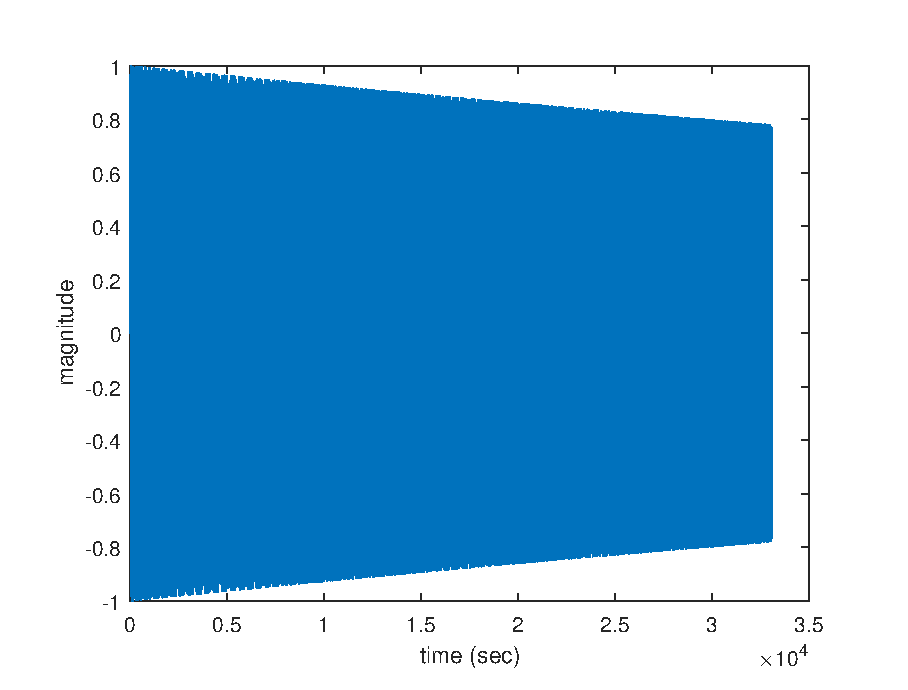
\includegraphics[scale=0.3]{time3}
		\caption{Time series plot of bell with the parameters $f_c = 110$, $f_m = 220$, $I_0 = 10$, $\tau = 12$, $T_{dur} = 3$, $f_s = 11025$}
	\end{minipage}
	\hspace{4cm}
	\begin{minipage}{0.3\linewidth}
		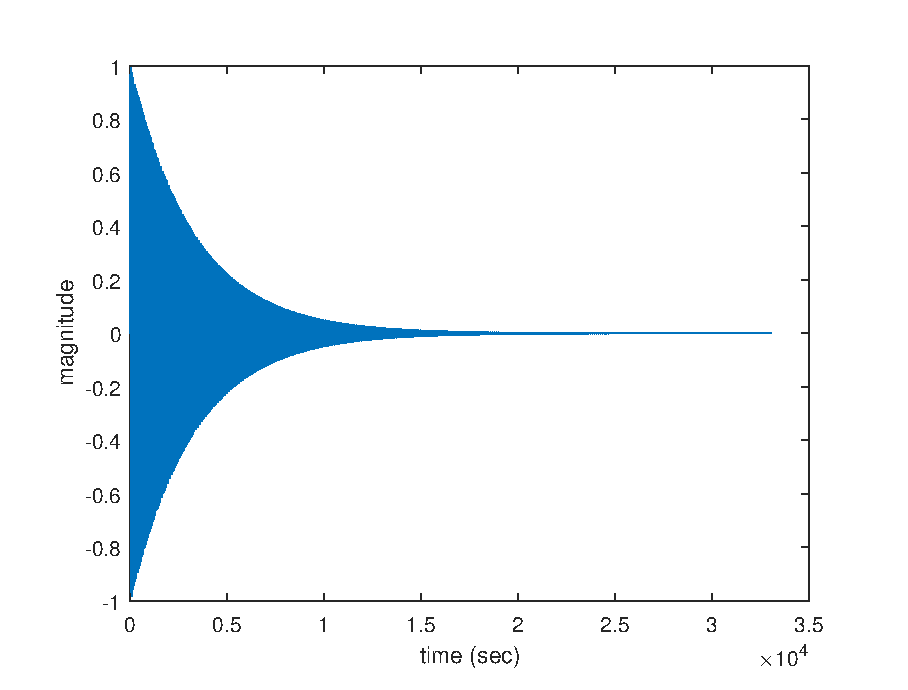
\includegraphics[scale=0.3]{time4}
		\caption{Time series plot of bell with the parameters $f_c = 110$, $f_m = 220$, $I_0 = 10$, $\tau = 0.3$, $T_{dur} = 3$, $f_s = 11025$}
	\end{minipage}
\end{figure}
\begin{figure}[H]
	\centering
	\begin{minipage}{0.3\linewidth}
		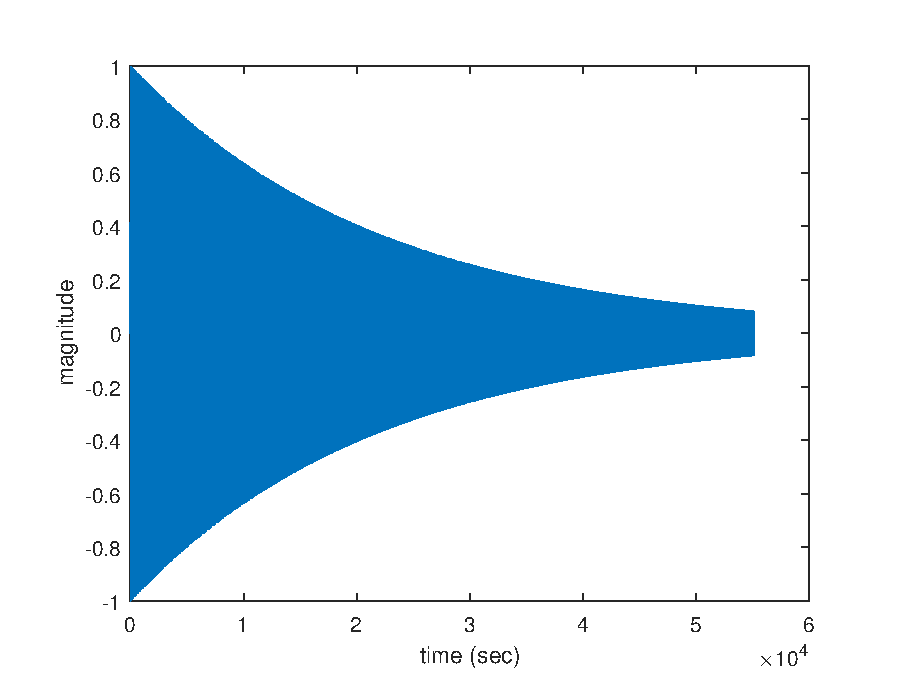
\includegraphics[scale=0.3]{time5}
		\caption{Time series plot of bell with the parameters $f_c = 250$, $f_m = 350$, $I_0 = 5$, $\tau = 2$, $T_{dur} = 5$, $f_s = 11025$}
	\end{minipage}
	\hspace{4cm}
	\begin{minipage}{0.3\linewidth}
		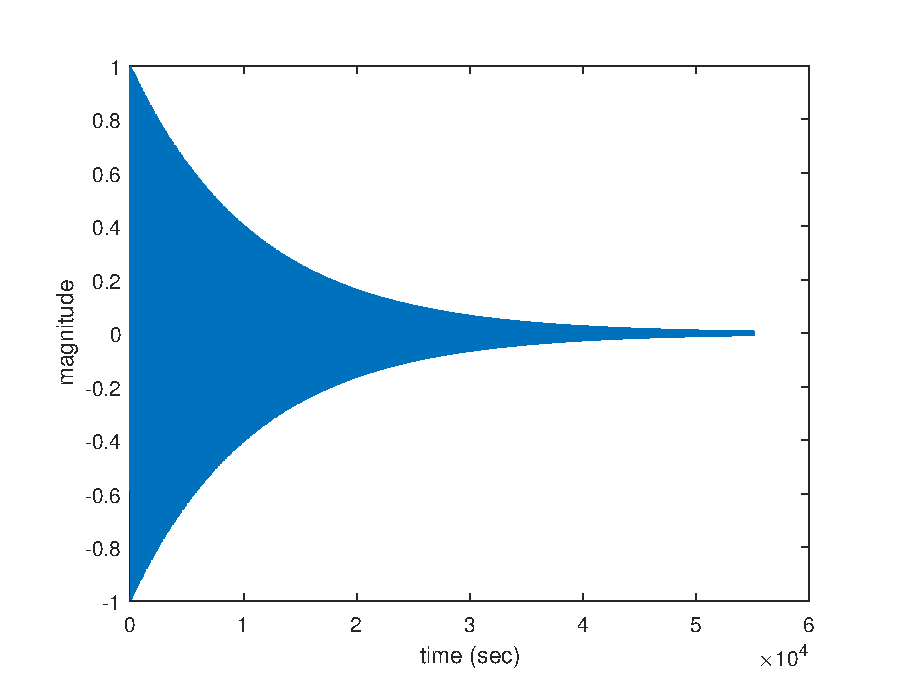
\includegraphics[scale=0.3]{time6}
		\caption{Time series plot of bell with the parameters $f_c = 250$, $f_m = 350$, $I_0 = 3$, $\tau = 1$, $T_{dur} = 5$, $f_s = 11025$}
	\end{minipage}
\end{figure}
\newpage
A spectrogram was created for each configuration of parameters a sound was played for - the spectrograms can be seen in Figures 13 through 18.
\begin{figure}[H]
	\centering
	\begin{minipage}{0.3\linewidth}
		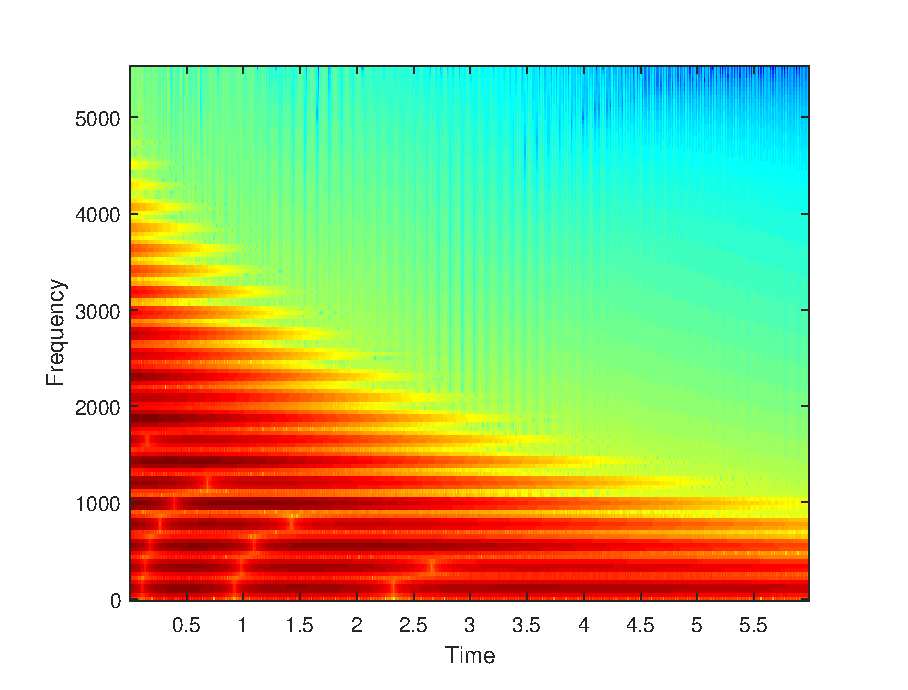
\includegraphics[scale=0.3]{spec1}
		\caption{Spectrogram of bell with the parameters $f_c = 110$, $f_m = 220$, $I_0 = 10$, $\tau = 2$, $T_{dur} = 6$, $f_s = 11025$}
	\end{minipage}
	\hspace{4cm}
	\begin{minipage}{0.3\linewidth}
		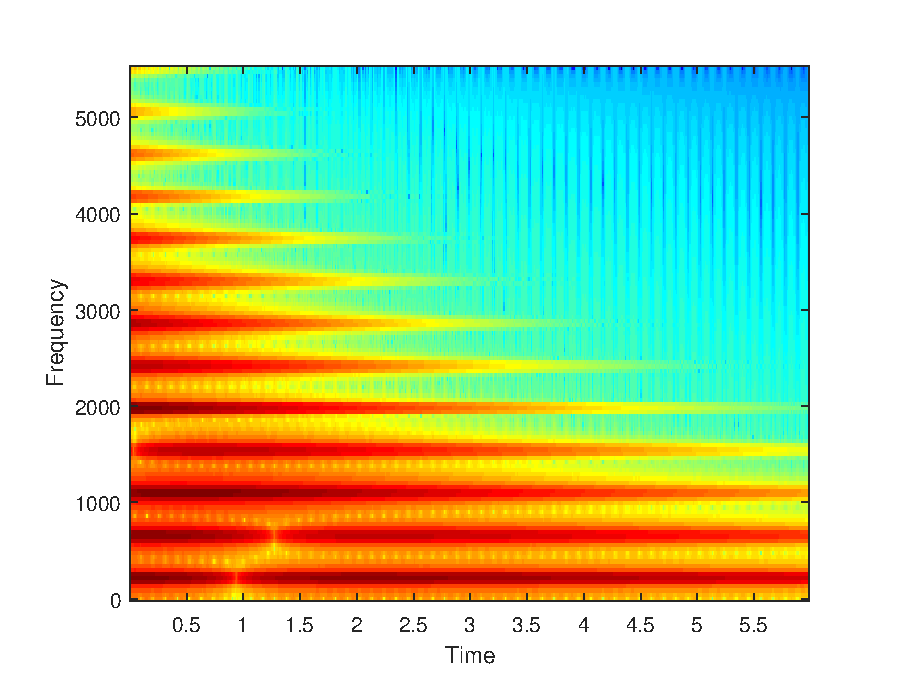
\includegraphics[scale=0.3]{spec2}
		\caption{Spectrogram of bell with the parameters $f_c = 220$, $f_m = 440$, $I_0 = 5$, $\tau = 2$, $T_{dur} = 6$, $f_s = 11025$}
	\end{minipage}
\end{figure}
\begin{figure}[H]
	\centering
	\begin{minipage}{0.3\linewidth}
		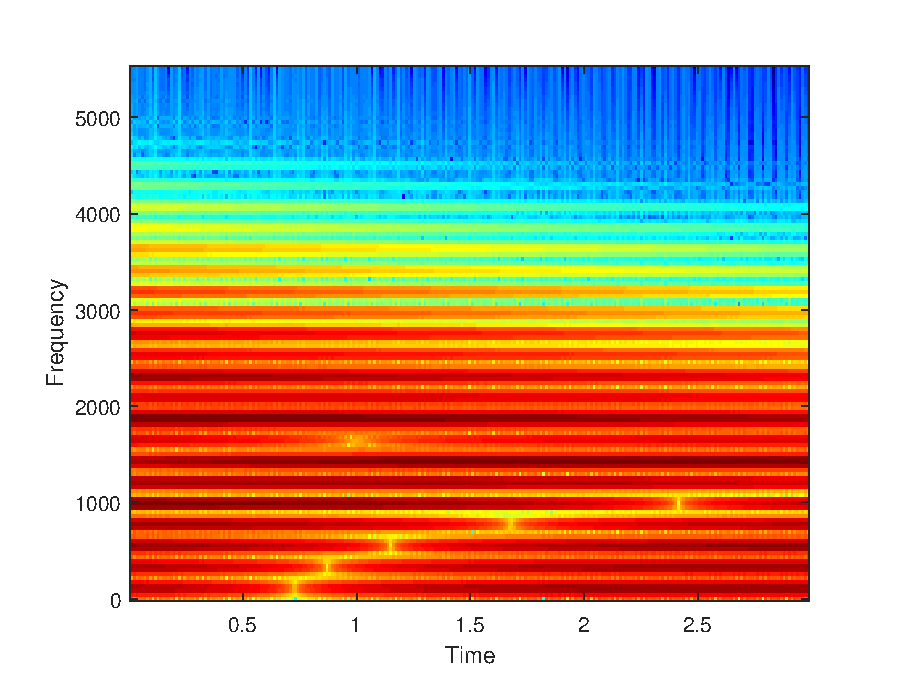
\includegraphics[scale=0.3]{spec3}
		\caption{Spectrogram of bell with the parameters $f_c = 110$, $f_m = 220$, $I_0 = 10$, $\tau = 12$, $T_{dur} = 3$, $f_s = 11025$}
	\end{minipage}
	\hspace{4cm}
	\begin{minipage}{0.3\linewidth}
		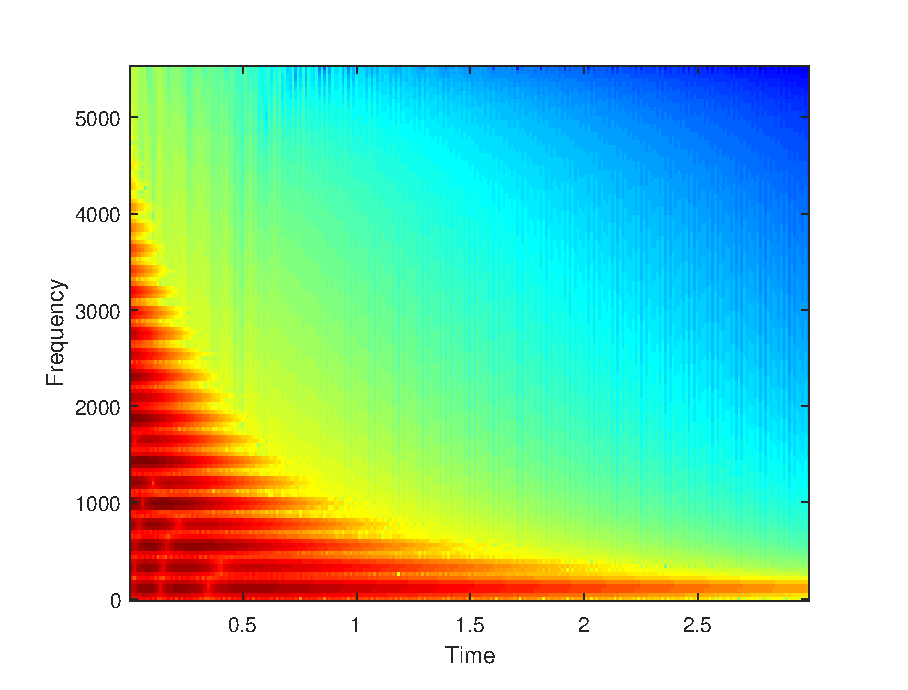
\includegraphics[scale=0.3]{spec4}
		\caption{Spectrogram of bell with the parameters $f_c = 110$, $f_m = 220$, $I_0 = 10$, $\tau = 0.3$, $T_{dur} = 3$, $f_s = 11025$}
	\end{minipage}
\end{figure}
\begin{figure}[H]
	\centering
	\begin{minipage}{0.3\linewidth}
		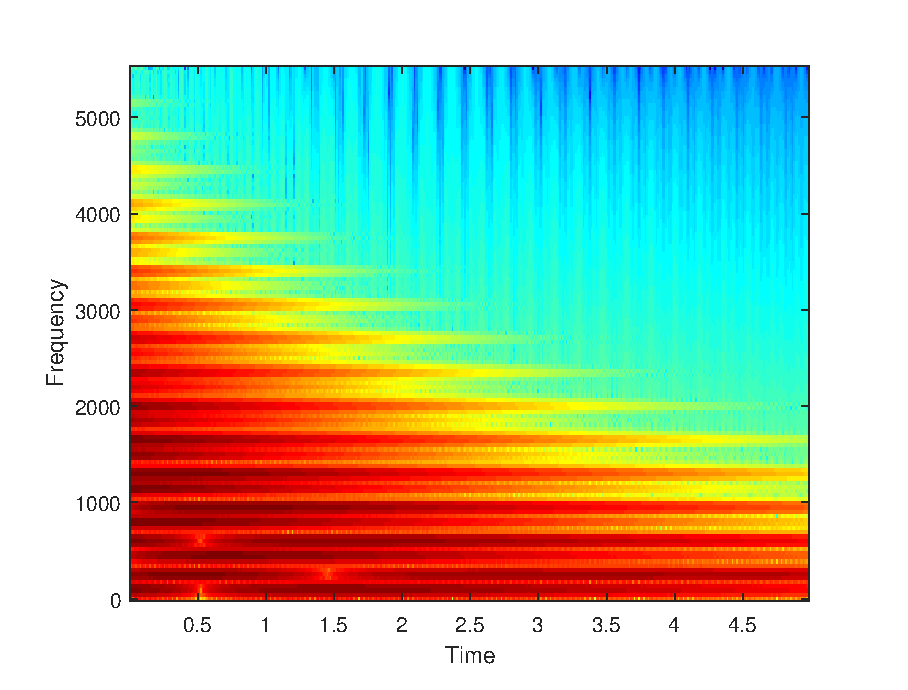
\includegraphics[scale=0.3]{spec5}
		\caption{Spectrogram of bell with the parameters $f_c = 250$, $f_m = 350$, $I_0 = 5$, $\tau = 2$, $T_{dur} = 5$, $f_s = 11025$}
	\end{minipage}
	\hspace{4cm}
	\begin{minipage}{0.3\linewidth}
		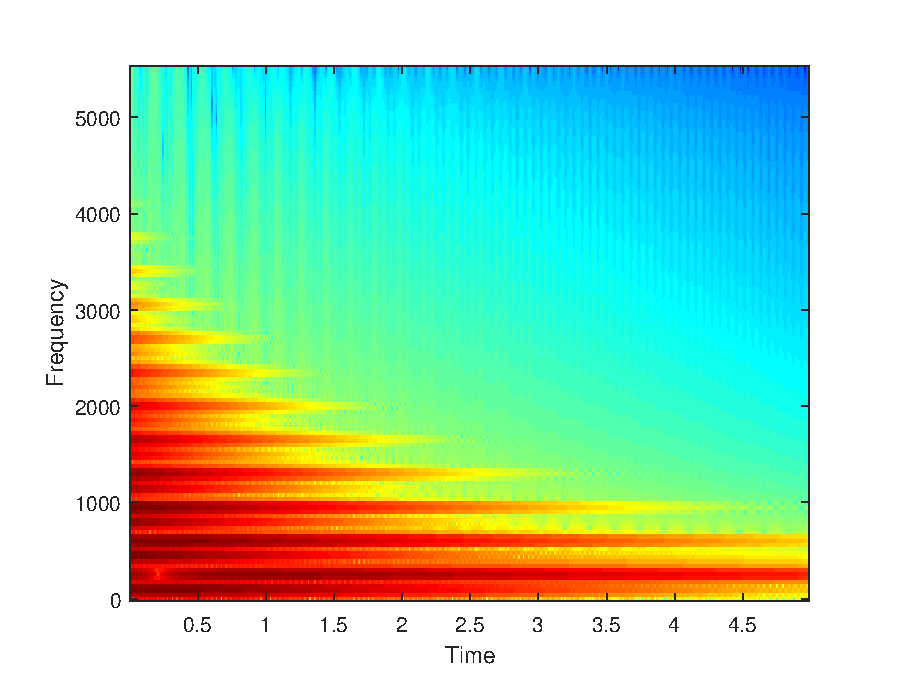
\includegraphics[scale=0.3]{spec6}
		\caption{Spectrogram of bell with the parameters $f_c = 250$, $f_m = 350$, $I_0 = 3$, $\tau = 1$, $T_{dur} = 5$, $f_s = 11025$}
	\end{minipage}
\end{figure}

Time series plots of the middle 300 samples of each of the bell signals for the parameter configuration were taken. The plots can be seen in Figures 19 through 24.
\begin{figure}[H]
	\centering
	\begin{minipage}{0.3\linewidth}
		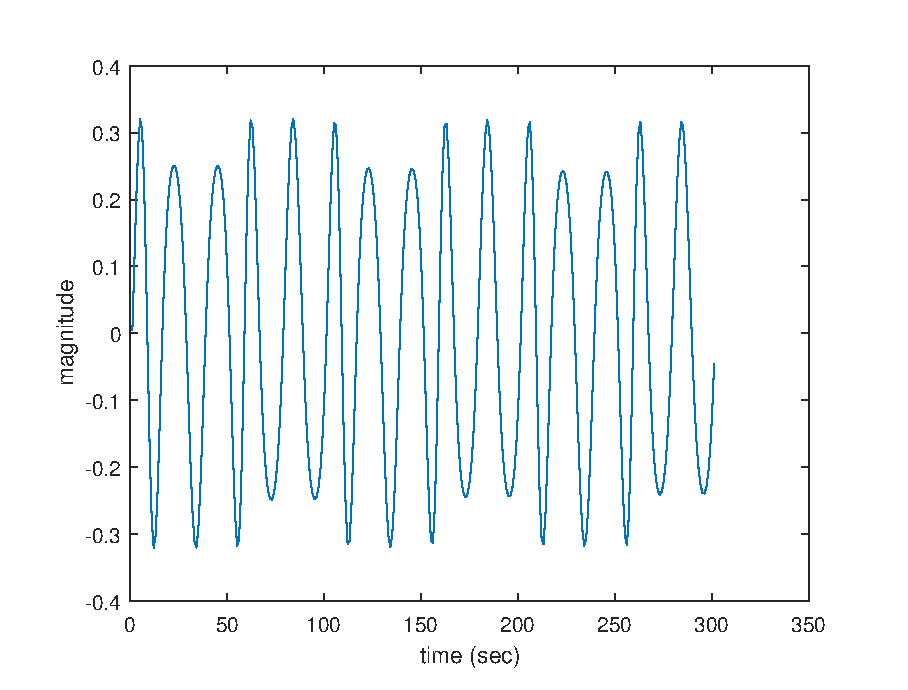
\includegraphics[scale=0.3]{samp1}
		\caption{300 samples of the time series plot of bell with the parameters $f_c = 110$, $f_m = 220$, $I_0 = 10$, $\tau = 2$, $T_{dur} = 6$, $f_s = 11025$}
	\end{minipage}
	\hspace{4cm}
	\begin{minipage}{0.3\linewidth}
		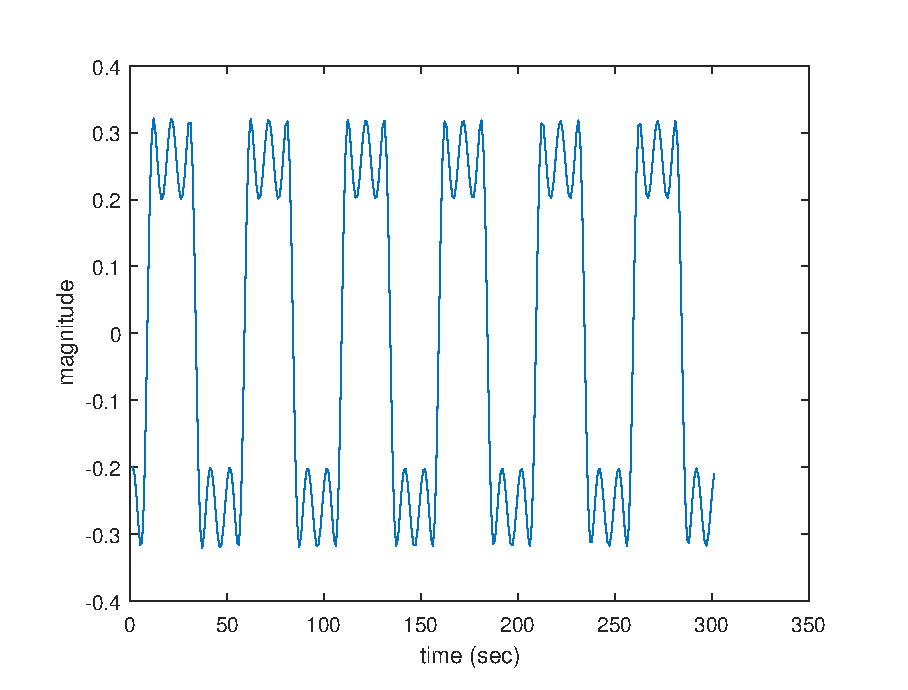
\includegraphics[scale=0.3]{samp2}
		\caption{300 samples of the time series plot of bell with the parameters $f_c = 220$, $f_m = 440$, $I_0 = 5$, $\tau = 2$, $T_{dur} = 6$, $f_s = 11025$}
	\end{minipage}
\end{figure}
\begin{figure}[H]
	\centering
	\begin{minipage}{0.3\linewidth}
		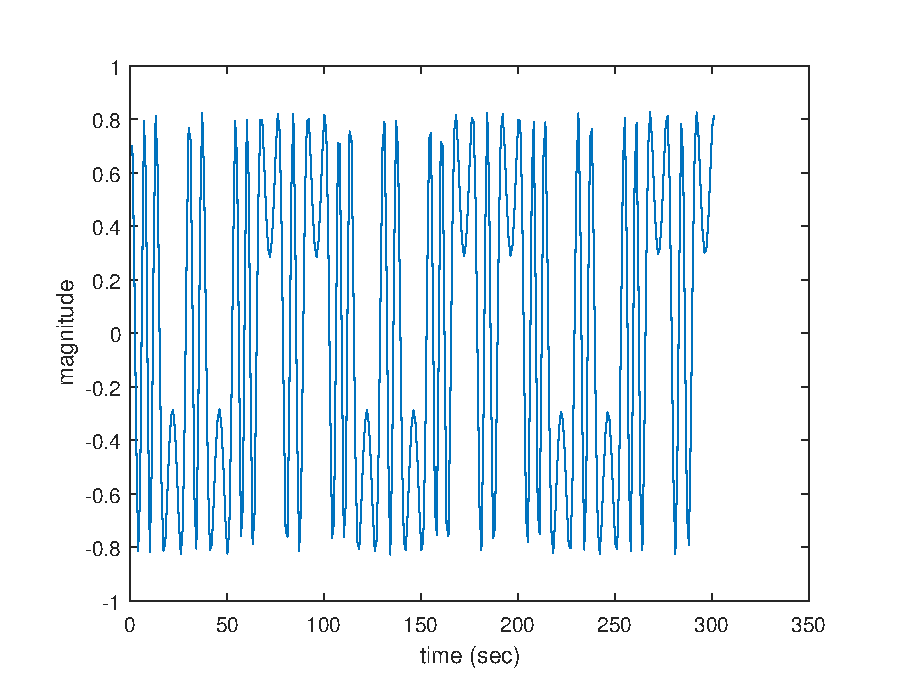
\includegraphics[scale=0.3]{samp3}
		\caption{Spectrogram of bell with the parameters $f_c = 110$, $f_m = 220$, $I_0 = 10$, $\tau = 12$, $T_{dur} = 3$, $f_s = 11025$}
	\end{minipage}
	\hspace{4cm}
	\begin{minipage}{0.3\linewidth}
		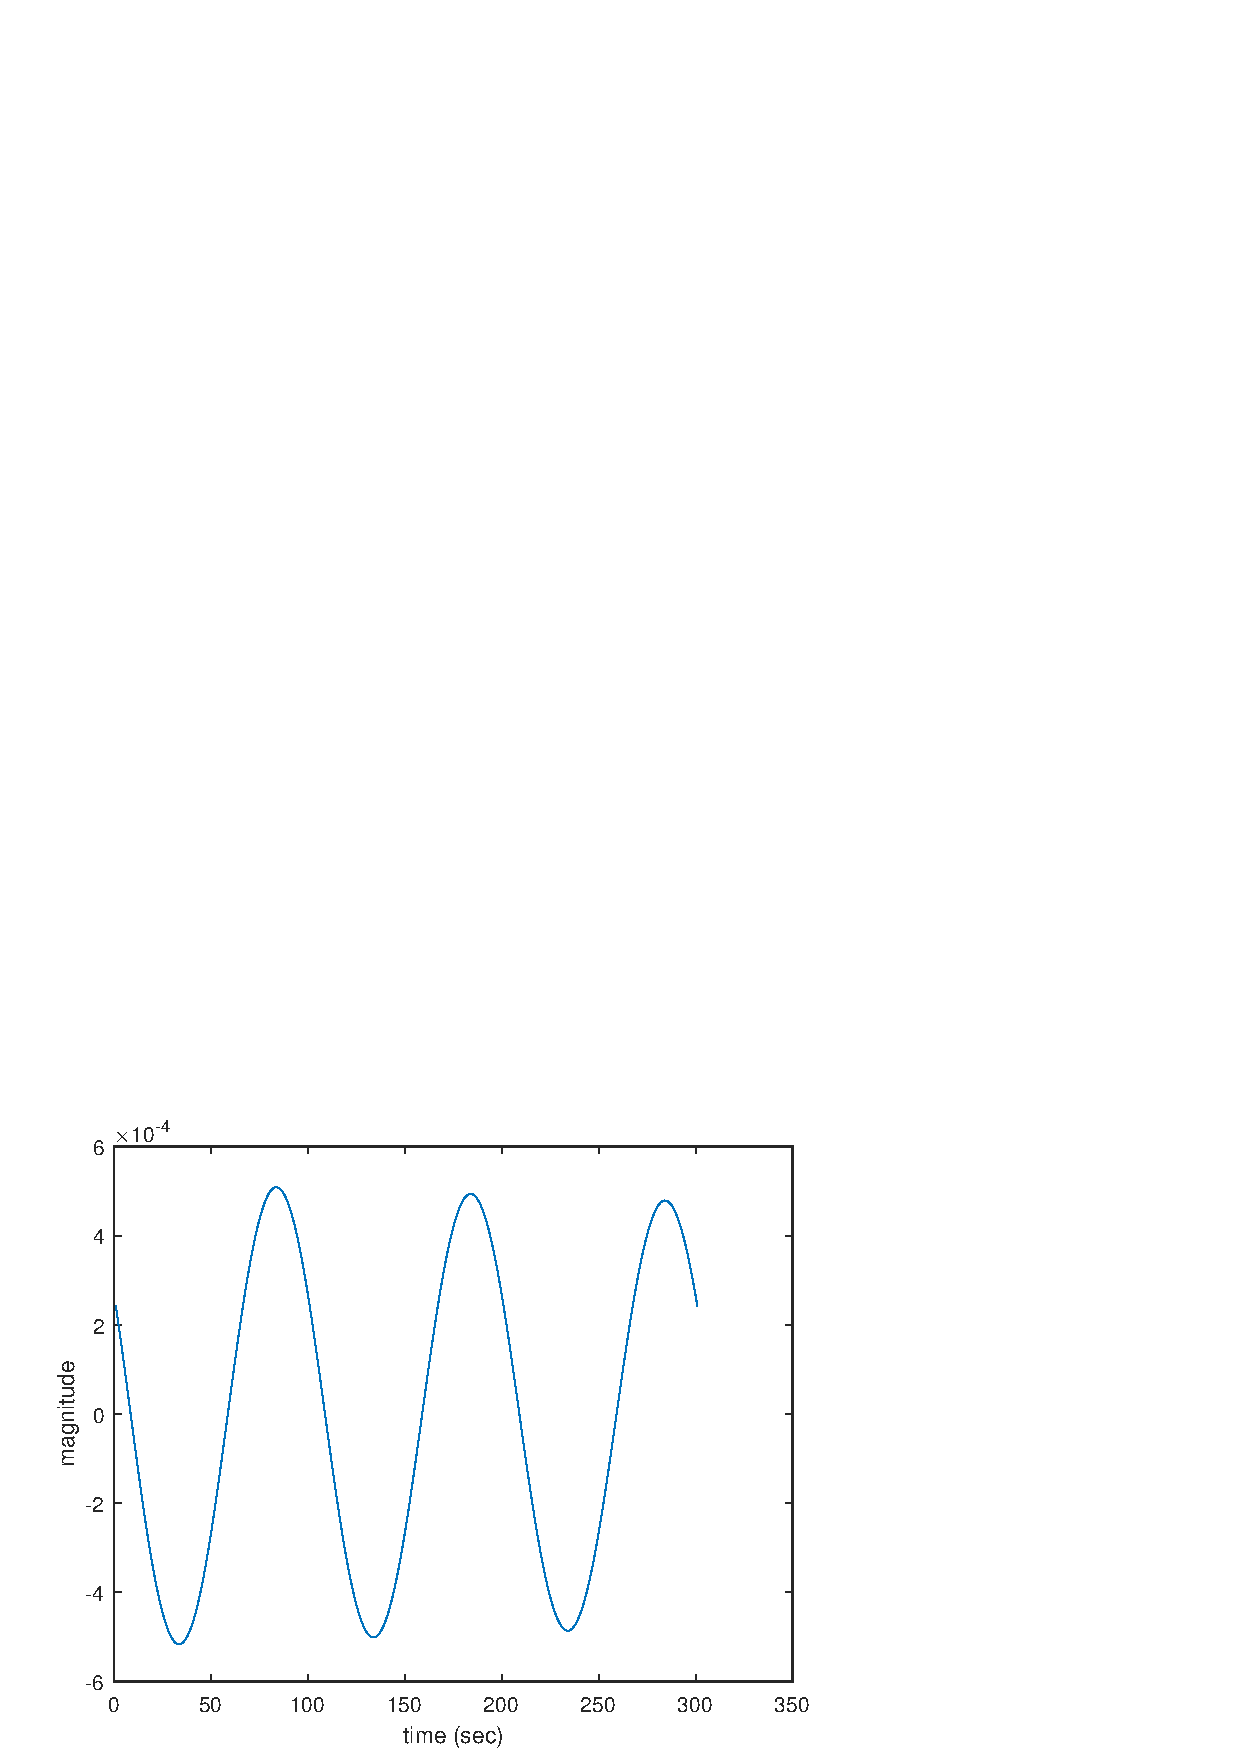
\includegraphics[scale=0.3]{samp4}
		\caption{300 samples of the time series plot of bell with the parameters $f_c = 110$, $f_m = 220$, $I_0 = 10$, $\tau = 0.3$, $T_{dur} = 3$, $f_s = 11025$}
	\end{minipage}
\end{figure}
\begin{figure}[H]
	\centering
	\begin{minipage}{0.3\linewidth}
		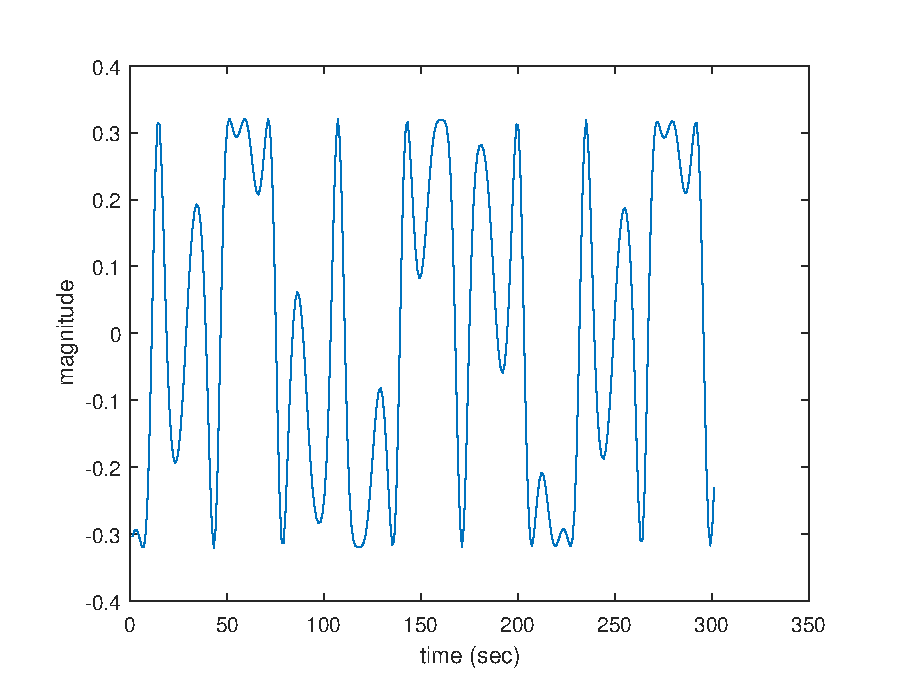
\includegraphics[scale=0.3]{samp5}
		\caption{300 samples of the time series plot of bell with the parameters $f_c = 250$, $f_m = 350$, $I_0 = 5$, $\tau = 2$, $T_{dur} = 5$, $f_s = 11025$}
	\end{minipage}
	\hspace{4cm}
	\begin{minipage}{0.3\linewidth}
		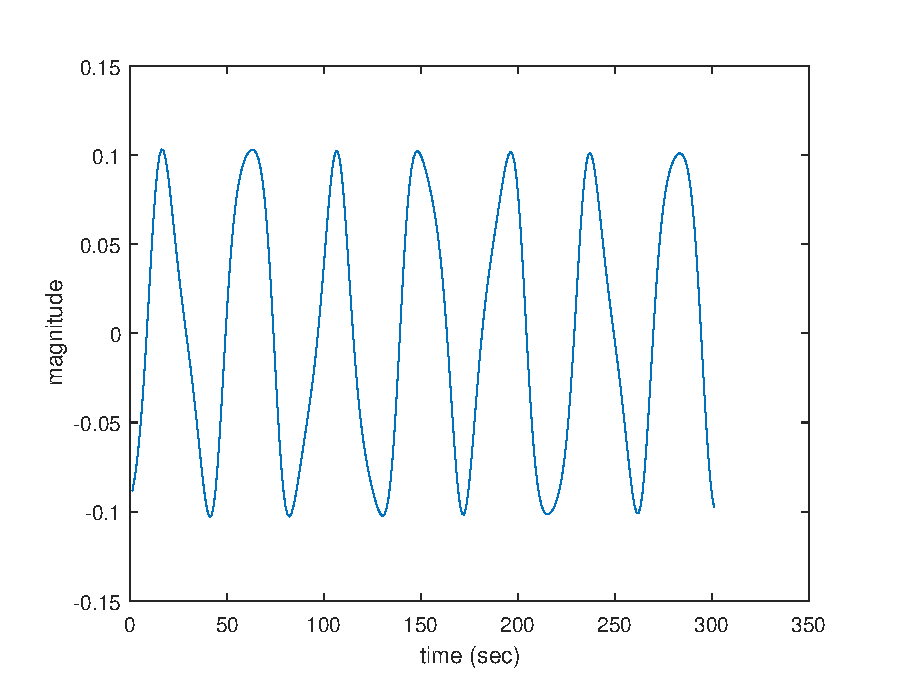
\includegraphics[scale=0.3]{samp6}
		\caption{300 samples of the time series plot of bell with the parameters $f_c = 250$, $f_m = 350$, $I_0 = 3$, $\tau = 1$, $T_{dur} = 5$, $f_s = 11025$}
	\end{minipage}
\end{figure}
\section{5.1 Generating the Envelopes for Woodwinds}
A function was provided which created the envelopes for Woodwind Synthesis, called \verb|woodwenv.m|, which produces the functions needed to create both $A(t)$ and $I(t)$. This was tested using the following script:
\begin{lstlisting}
	%%%%%%%%% 5.1 Generating the Envelopes for Woodwinds %%%%%%%%%%%%
	
	% Clear the work space and any stored variables
	clear; clc;
	
	fsamp = 8000;
	Ts = 1/fsamp;
	delta = 1e-4;
	tt = delta:Ts:0.5;
	[y1, y2] = woodwenv(0.1, 0.35, 0.05, fsamp);
	subplot(2,1,1), plot(tt,y1), grid on
	subplot(2,1,2), plot(tt,y2), grid on
\end{lstlisting}

\section{5.2 Scaling the Clarinet Envelopes}
Scaling of the envelope functions was required. A linear mapping was used to scale normalised envelope values, seen below:
\begin{align*}
	y_{new}(t) = \alpha \cdot y_{norm}(t) + \beta
\end{align*}

The section asks (seemingly as busy work) to map the normalised value of 1 to $(y_{new})_{max}$ and the normalised value of 0 to $(y_{new})_{min}$. If $y_{norm} = 0$, then:
\begin{align*}
	(y_{new})_{min} = \alpha \cdot 0 + \beta = \beta
\end{align*}

Similarly, if $y_{norm} = 1$, then:
\begin{align*}
	(y_{new})_{max} = \alpha \cdot 1 + \beta = \alpha + (y_{new})_{min}
\end{align*}

Hence, we have that $\beta = (y_{new})_{min}$, and $\alpha = (y_{new})_{max} - (y_{new})_{min}$, in order to create the desired linear mapping outlined in the exercise. A function was used to implement the scaling operation in MATLAB, which can be seen below:
\begin{lstlisting}
	function y = scale(data, alpha, beta)
	    y = alpha*data + beta;
	end
\end{lstlisting}

\section{5.3 Clarinet Envelopes}
The $I(t)$ clarinet envelope needs to be scaled, and inverted. In this instance, the profile that is provided sees the normalised value of 0 mapped to 4, and the normalised value of 1 is mapped to 2. Applying a similar logic to the previous exercise, we see that if $y_{norm} = 0$, then:
\begin{align*}
	(y_{new})_{max} = 4 = \alpha \cdot 0 + \beta
\end{align*}

Similarly, if $y_{norm} = 1$, then:
\begin{align*}
	(y_{new})_{min} = 2 = \alpha \cdot 1 + \beta = \alpha + 4
\end{align*}

Hence, we see that we should set the parameters as $\alpha = -2$, and $\beta = 4$. This was implemented using the following script:
\begin{lstlisting}
	%%%%%%%%%%%%%% 5.3 Clarinet Envelopes %%%%%%%%%%%%%%%%%%%%%%
	beta = 4;
	alpha = 2 - beta;
	
	fsamp = 8000;
	Ts = 1/fsamp;
	delta = 1e-4;
	tt = delta:Ts:0.5;
	[y1, y2] = woodwenv(0.1, 0.35, 0.05, fsamp);
	
	I = scale(y2,alpha,beta);
\end{lstlisting}

\section{5.4 Parameters for the Clarinet}
A MATLAB function was implemented to create the signal for a clarinet, noting that the fundamental frequency, $f_0$, is used to derive the carrier and modulation frequencies $f_c$ and $f_m$, respectively. The section asks the envelopes $A(t)$ and $I(t)$ to be implemented using the functions \verb|textttscale| and \verb|textttwoodwenv|, however, these functions were not available. The previously defined functions \verb|scale| and \verb|woodwenv| were employed instead. The function is as follows:
\begin{lstlisting}
	function yy = clarinet(f0, Aenv, Ienv, dur, fsamp)
	%CLARINET produce a clarinet note signal
	% usage: yy = clarinet(f0, Aenv, Ienv, dur, fsamp)
	% where:
	% f0 = note frequency
	% Aenv = the array holding the A(t) envelope
	% Ienv = the array holding the I(t) envelope
	% dur = the amount of time the signal lasts
	% fsamp = the sampling rate
	    
	    % Create time vector
	    tt = 1e-4:(1/fsamp):dur;
	    
	    % Set up alpha and beta for use in scaling function
	    alpha = -2;
	    beta = 4;
	    
	    % Scale the I(t) envelope
	    I_new = scale(Ienv,alpha,beta);
	    
	    % Determine the fc and fm parameters
	    fc = 2*f0;
	    fm = 3*f0;
	    phm = -pi/2;
	    phc = -pi/2;
	    
	    % Create the clarinet sound
	    arg = 2*pi*fc*tt + I_new.*real(exp(j*(2*pi*fm*tt + phm))) + phc;
	    yy = Aenv.*real(exp(j*arg));
	end
\end{lstlisting}

\section{5.5 Experiment with the Clarinet Sound}
The clarinet sound was tested using the following script:
\begin{lstlisting}
	%%%%%%%%%%%%%%%%%% 5.5 Experiment with Clarinet Sound %%%%%%%%%%%%%%%%%%
	
	% Clear the workspace and any stored variables
	clear; clc;
	
	% Set the parameters for the sound
	f0 = 290;
	
	% Set the duration of the tone
	dur = 2;
	
	% Set the sampling frequency
	fsamp = 8000;
	
	% Create the envelopes for the sound
	a = (0.1/0.5)*2; s = (0.35/0.5)*2; r = (0.05/0.5)*2;
	[Aenv, Ienv] = woodwenv(a, s, r, fsamp);
	
	% Build the discrete time waveform
	xx = clarinet(f0, Aenv, Ienv, dur, fsamp);
	
	% Play the sound
	sound(xx,fsamp)
\end{lstlisting}

The generated sound is roughly like a woodwind instrument at lower frequencies. Higher frequencies sound artificial.
\end{document}
